\section{Distributed join and scaling (RQ2)}
\label{results:distributed-join-and-scaling}

% ORIENTING COMMENT (section intro prose -- TODO below). One paragraph, no
%   numbers: present the national-scale spatial join run on Apache Sedona
%   (Databricks) across worker counts {2, 4, 8, 12, 16} and the two execution
%   strategies (broadcast and partitioned), against the single-node PostGIS and
%   DuckDB baselines, at the small/medium/large tiers. Present, in order: scaling
%   behavior, absolute performance vs. the single-node baselines, the
%   execution-phase breakdown, then cost and the cost-time tradeoff. Results only;
%   interpretation is deferred to the Discussion (Chapter~\ref{ch:discussion}).

% TODO (prose): section-opening paragraph per the orienting comment above.

\subsection{Scaling behavior}
\label{results:distributed-join-and-scaling:scaling-behavior}

% TODO (prose): factual readout only of speedup and parallel efficiency -- the
% curve shapes and where they depart from ideal. Refer to
% Figure~\ref{fig:distributed-speedup-efficiency}. No interpretation (-> Discussion).

\begin{figure}[H]
    \centering
    % WHAT IT SHOWS: two-panel scaling float over worker counts {2, 4, 8, 12, 16}.
    %   (a) speedup S(n) = T_2 / T_n, one series for broadcast and one for
    %       partitioned, with an ideal-linear reference S(n) = n/2 (baseline is
    %       the 2-worker cluster).
    %   (b) paired parallel efficiency E(n) = (2/n) * S(n), same two series, with
    %       the ideal E(n) = 1 reference.
    % CAPTION MUST STATE: the worker-count axis; that speedup and efficiency are
    %   defined relative to the 2-worker baseline (n0 = 2) per
    %   Equation~\ref{eq:speedup-parallel-efficiency}; the two strategies; and the
    %   ideal reference in each panel.
    % DESCRIPTIVE ONLY: report the curves; no interpretation (-> Discussion).
    \subfloat[Speedup $S(n)$.\label{fig:distributed-speedup}]{%
        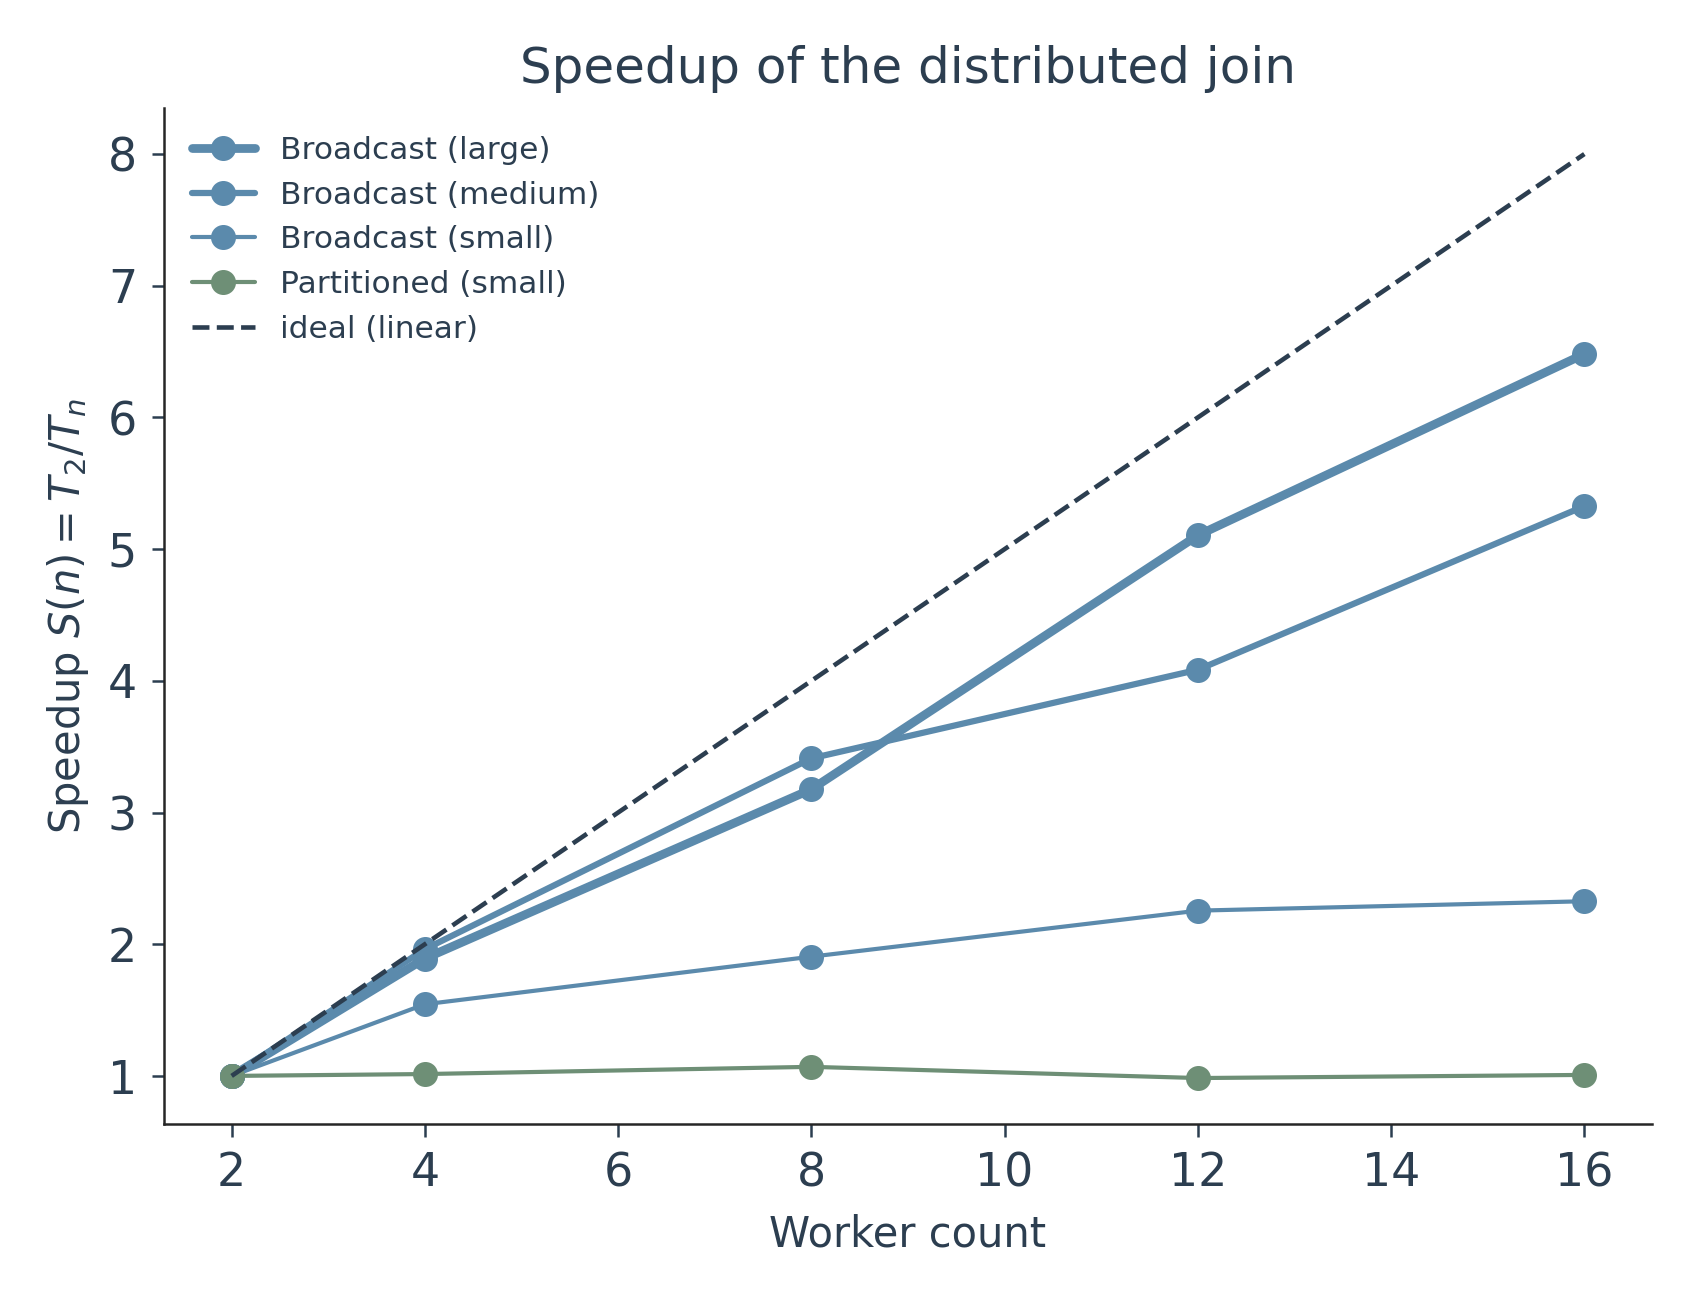
\includegraphics[valign=t, width=0.45\textwidth]{Chapters/06-results/sub-chapters/figures/06-distributed-speedup.png}}%
    \hfill
    \subfloat[Parallel efficiency $E(n)$.\label{fig:distributed-efficiency}]{%
        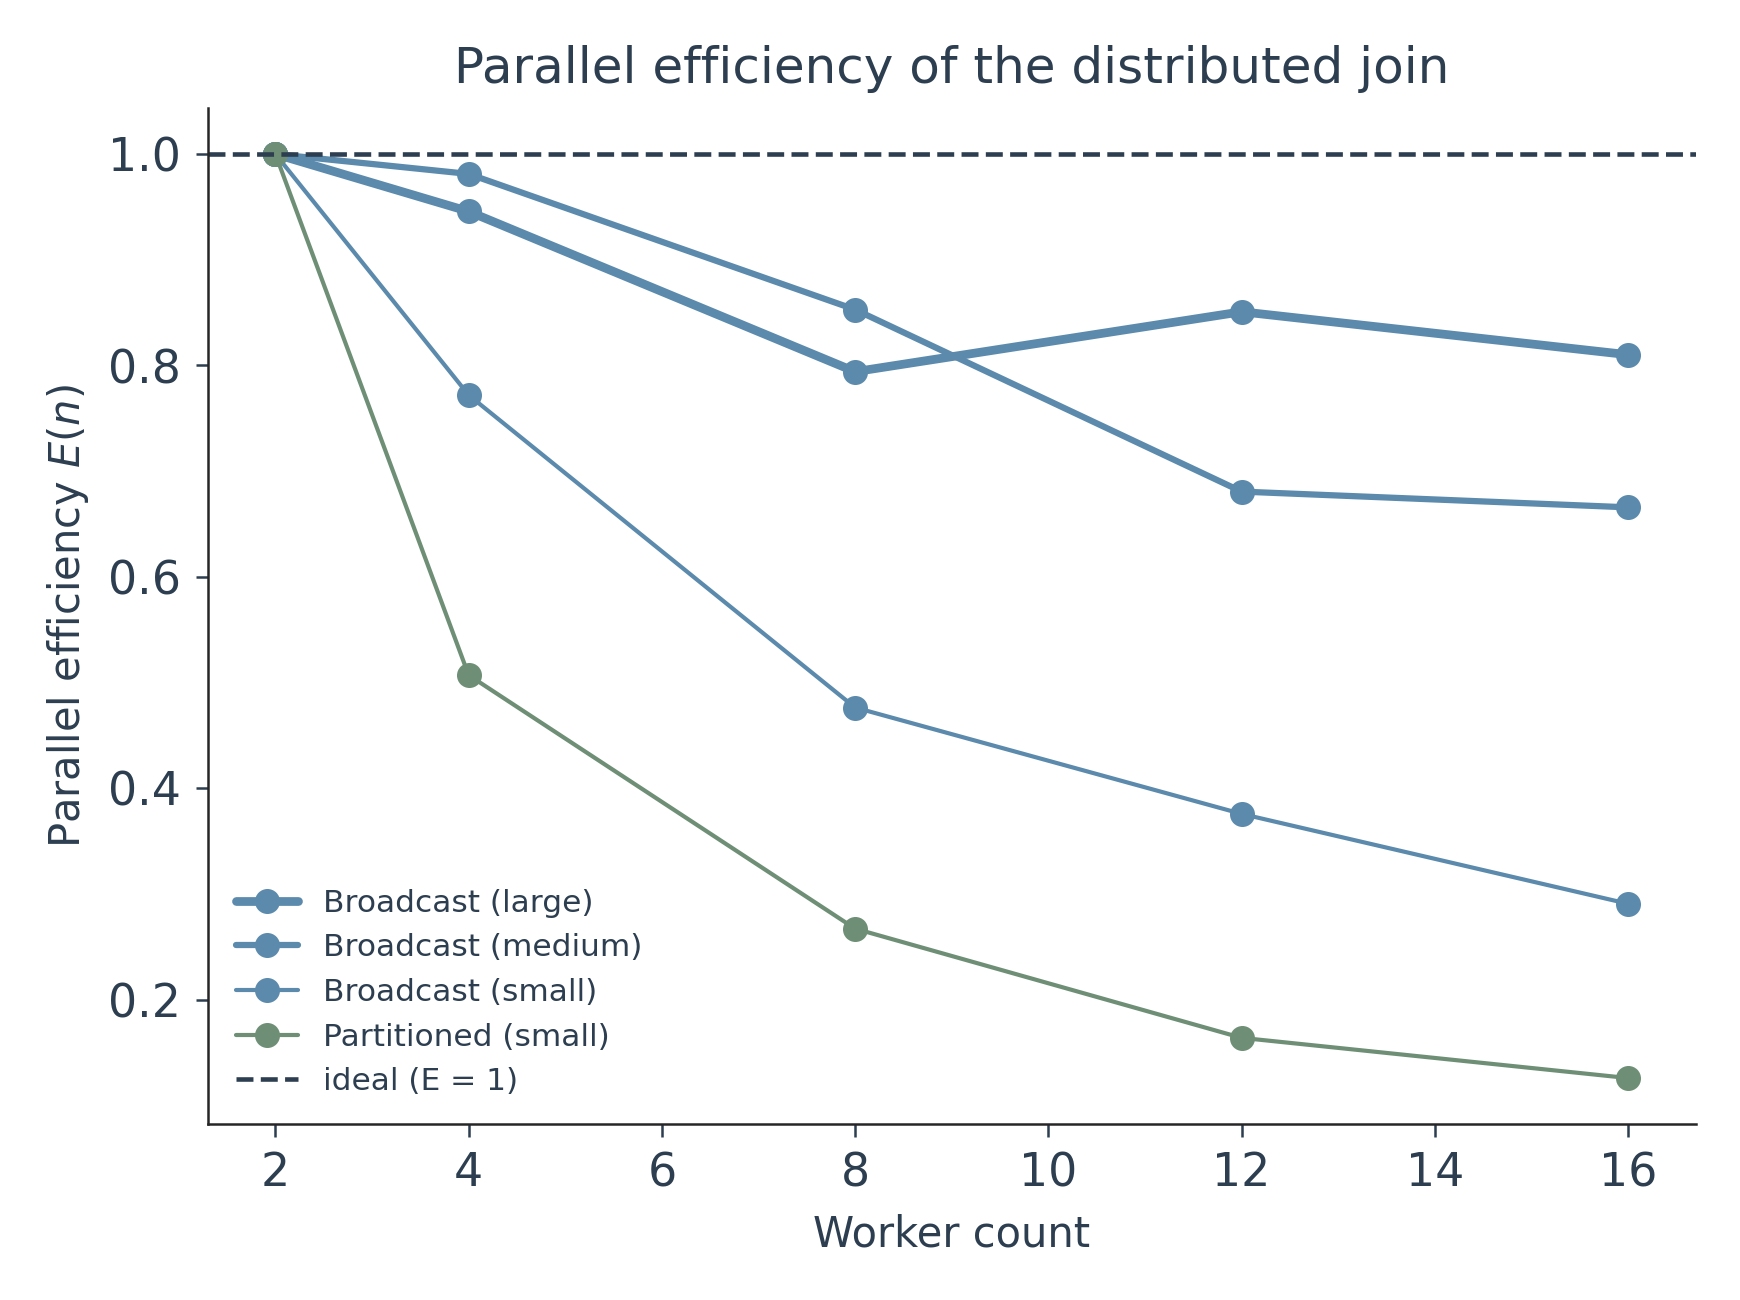
\includegraphics[valign=t, width=0.45\textwidth]{Chapters/06-results/sub-chapters/figures/06-distributed-efficiency.png}}%
    \caption[Speedup and parallel efficiency of the distributed join]{Scaling of
    the distributed spatial join over worker counts $\{2, 4, 8, 12, 16\}$, defined
    relative to the two-worker baseline ($n_0 = 2$) of
    Equation~\ref{eq:speedup-parallel-efficiency}. Panel~(a) shows speedup
    $S(n) = T_2/T_n$ for the broadcast and partitioned strategies against an
    ideal-linear reference; panel~(b) shows the paired parallel efficiency
    $E(n) = (2/n)\,S(n)$ against its ideal of one. Series colour encodes join
    strategy and the reference line uses a neutral palette colour.}
    \label{fig:distributed-speedup-efficiency}
\end{figure}

\subsection{Absolute performance vs. single-node baselines}
\label{results:distributed-join-and-scaling:absolute-performance-vs-single-node-baselines}

% TODO (prose): factual readout only -- absolute wall-clock at each worker count
% against the PostGIS and DuckDB baselines, and the worker count (if any, within
% 2--16) at which the distributed join first overtakes the best single-node
% engine. Refer to Figure~\ref{fig:distributed-wall-clock-vs-workers}. No
% interpretation (-> Discussion).

\begin{figure}[H]
    \centering
    % WHAT IT SHOWS: wall-clock time (minimum estimator) against worker count
    %   {2, 4, 8, 12, 16} for the distributed join, with the single-node PostGIS
    %   and DuckDB baselines drawn as horizontal reference lines, and the crossover
    %   point -- where the distributed curve first drops below the best single-node
    %   baseline -- explicitly marked (or stated as "no crossover within 2--16").
    % CAPTION MUST STATE: the axes; that baselines are horizontal single-node
    %   reference lines; that the crossover is marked; the tier shown; the
    %   estimator.
    % STRATEGY: treat the broadcast/partitioned dimension consistently -- either
    %   plot both strategies, or pick the winning strategy and SAY SO in the
    %   caption. Keep this choice consistent with the speedup figure.
    % DESCRIPTIVE ONLY: report the crossover location; no interpretation.
    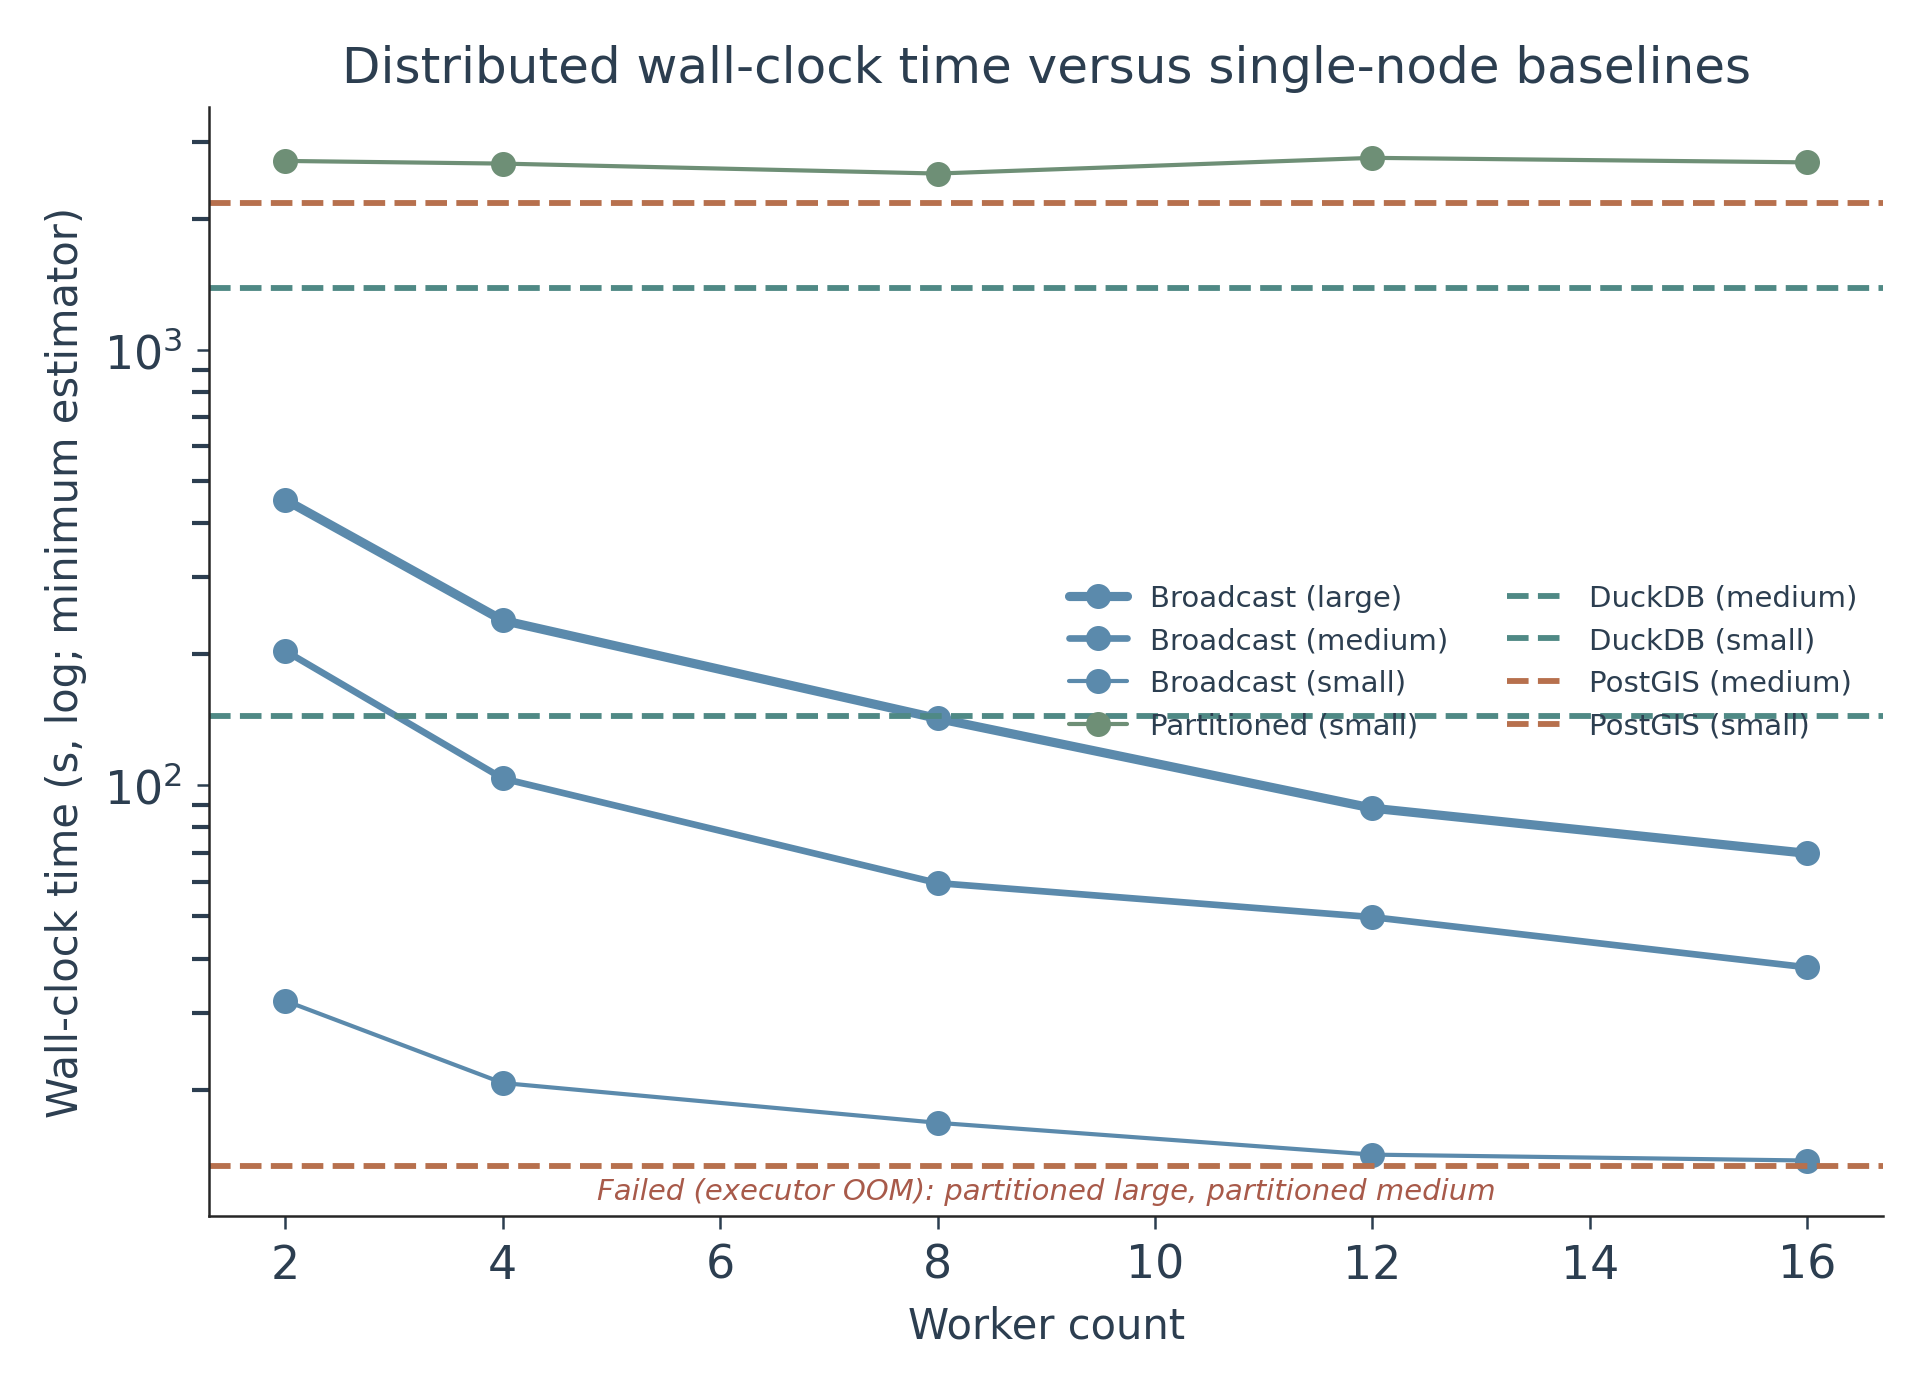
\includegraphics[width=0.8\textwidth]{Chapters/06-results/sub-chapters/figures/06-distributed-wall-clock-vs-workers.png}
    \caption[Distributed wall-clock time versus single-node baselines]{Wall-clock
    time of the distributed join as a function of worker count, with the
    single-node PostGIS and DuckDB baselines shown as horizontal reference lines.
    The worker count at which the distributed join first overtakes the best
    single-node baseline is marked as the crossover point. Bar/line height is the
    minimum-estimator elapsed time; the join strategy shown is stated consistently
    with the scaling figure.}
    \label{fig:distributed-wall-clock-vs-workers}
\end{figure}

\subsection{Execution-phase breakdown}
\label{results:distributed-join-and-scaling:execution-phase-breakdown}

% TODO (prose): factual readout only of where the distributed time and bytes go
% across phases, vs. worker count. Refer to
% Figure~\ref{fig:distributed-execution-phase-breakdown}. No interpretation.

\begin{figure}[H]
    \centering
    % WHAT IT SHOWS: two-panel execution-phase breakdown vs. worker count, using
    %   the three phases of the distributed lifecycle as instrumented
    %   (Section~\ref{research-design-and-methodology:metrics-and-cost-model:distributed-phase-metrics}):
    %   executor read time, shuffle, and driver collection.
    %   (a) stacked wall-clock time across executor-read / shuffle / driver-collection,
    %       per worker count (and strategy);
    %   (b) shuffle bytes across the same worker counts (and strategy).
    % CAPTION MUST STATE: the three phases by their instrumented names
    %   (executor read time, shuffle, driver collection -- driver collection is the
    %   clamped residual); the axes; that panel (b) is shuffle bytes.
    % DESCRIPTIVE ONLY: report the stacks; no interpretation (-> Discussion).
    \subfloat[Wall-clock time by phase.\label{fig:distributed-phase-time}]{%
        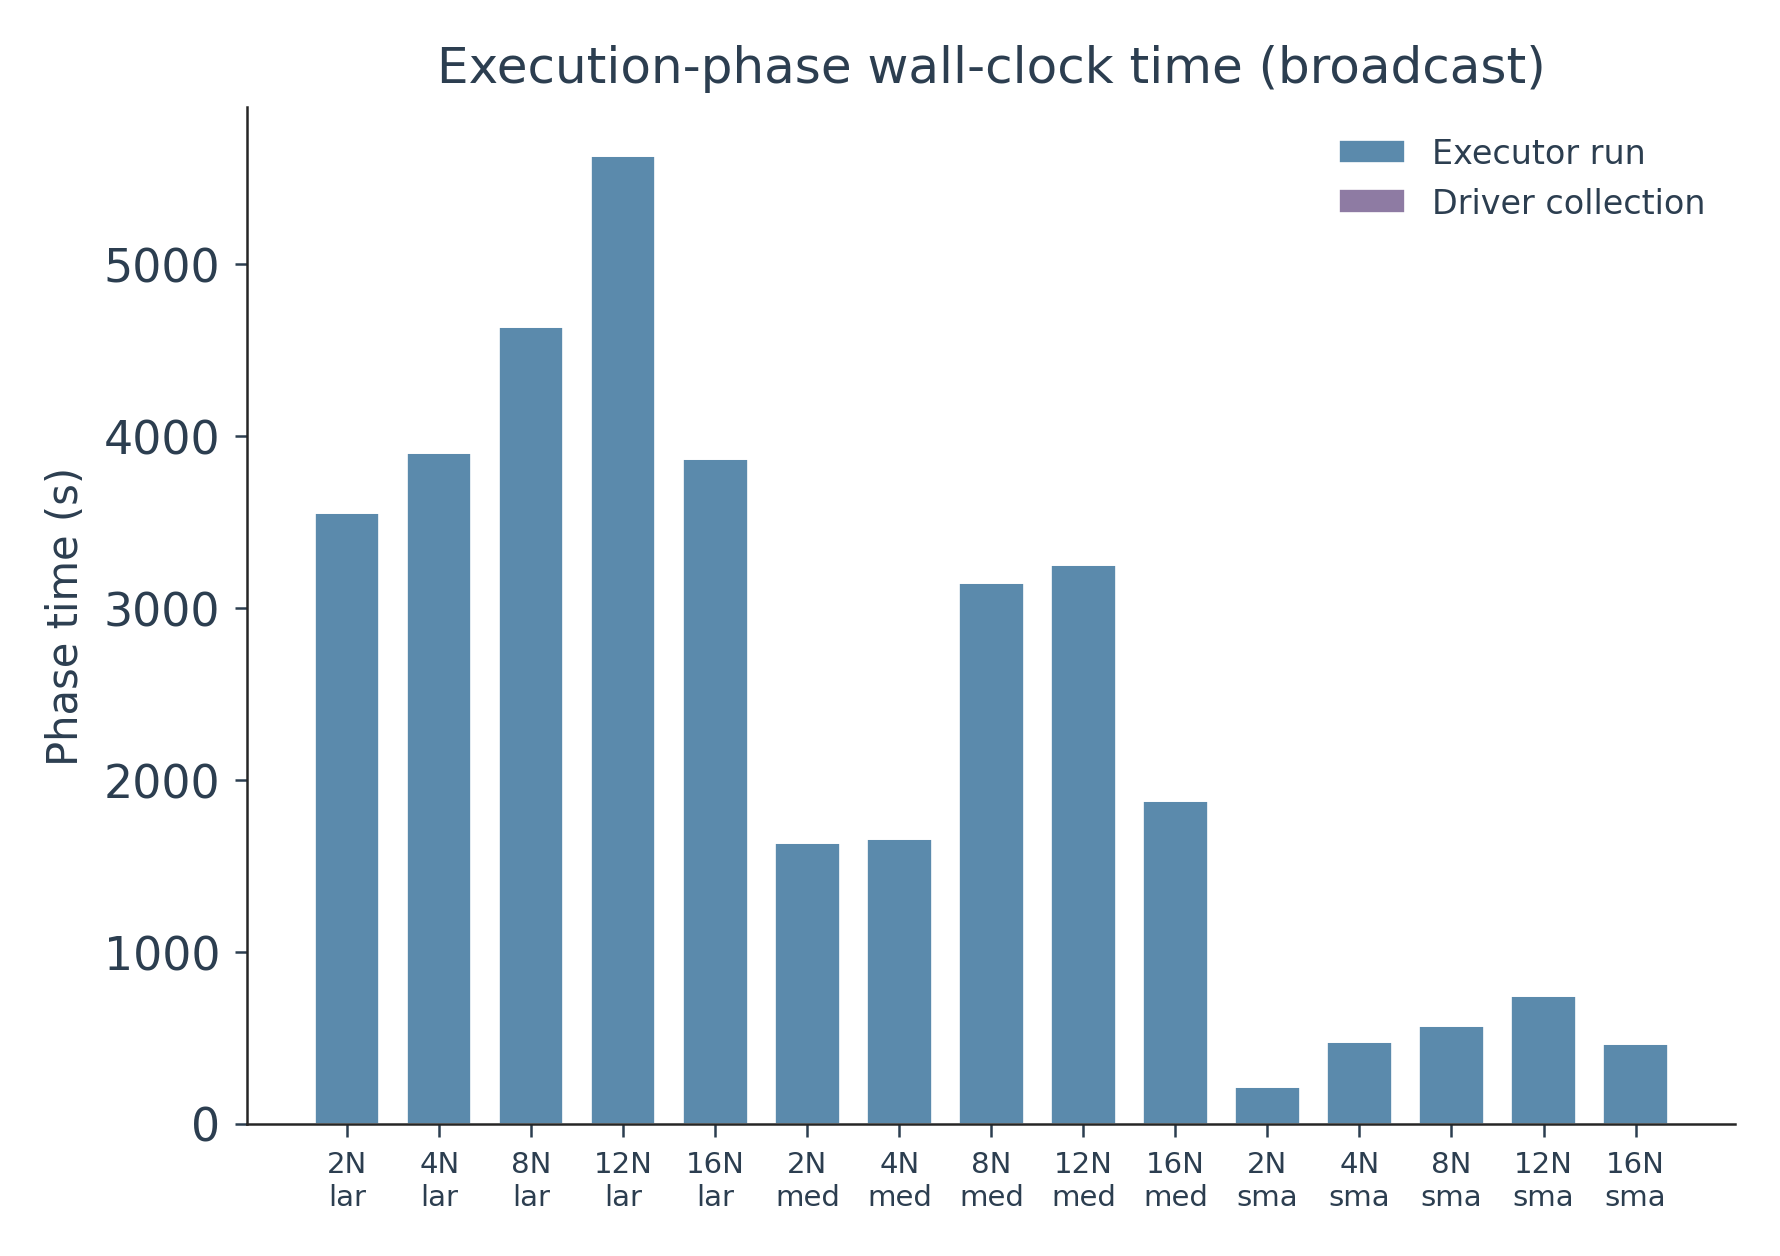
\includegraphics[valign=t, width=0.45\textwidth]{Chapters/06-results/sub-chapters/figures/06-distributed-phase-time.png}}%
    \hfill
    \subfloat[Shuffle bytes.\label{fig:distributed-shuffle-bytes}]{%
        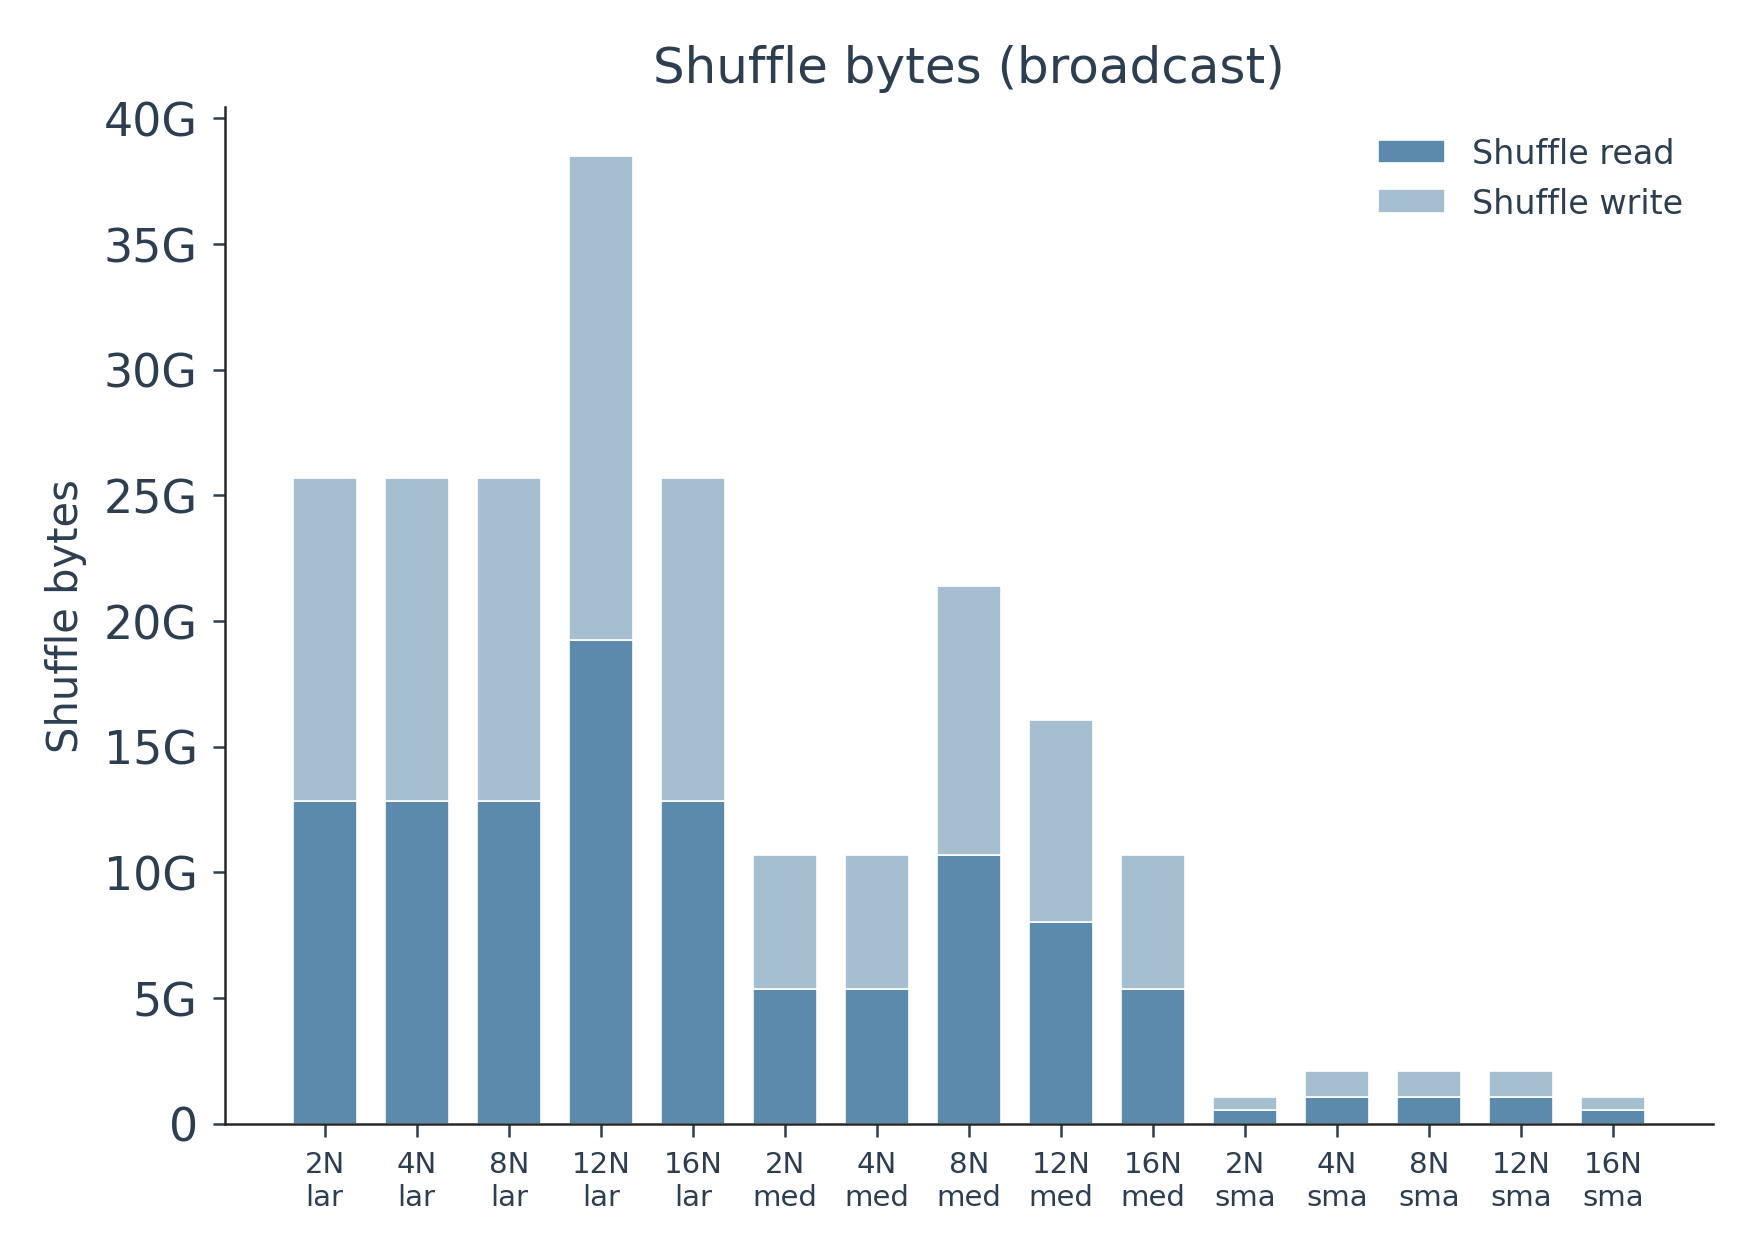
\includegraphics[valign=t, width=0.45\textwidth]{Chapters/06-results/sub-chapters/figures/06-distributed-shuffle-bytes.png}}%
    \caption[Execution-phase breakdown of the distributed join]{Decomposition of
    the distributed join across the three instrumented phases of the distributed
    lifecycle -- executor read time, shuffle, and driver collection (the last
    recovered as the clamped wall-clock residual). Panel~(a) stacks wall-clock
    time by phase against worker count; panel~(b) shows the corresponding shuffle
    bytes. Phase colour uses the thesis palette.}
    \label{fig:distributed-execution-phase-breakdown}
\end{figure}

\subsection{Operational cost and the cost-time tradeoff}
\label{results:distributed-join-and-scaling:operational-cost-and-the-cost-time-tradeoff}

% TODO (prose): factual readout only of cost vs. time across worker counts, and
% which points lie on the frontier. Refer to
% Figure~\ref{fig:distributed-cost-time-pareto} and
% Table~\ref{tab:distributed-join-descriptive-statistics}. No interpretation.

\begin{figure}[H]
    \centering
    % WHAT IT SHOWS: cost-time Pareto scatter. One point per worker count
    %   {2, 4, 8, 12, 16} in (wall-clock time, operational cost) space, a separate
    %   series for broadcast and partitioned; the non-dominated points are joined
    %   to trace the Pareto frontier.
    % CAPTION MUST STATE: the two axes (time, cost); that each point is one worker
    %   count; the two strategies; and that the frontier is the non-dominated set.
    % DESCRIPTIVE ONLY: report which points are non-dominated; no interpretation.
    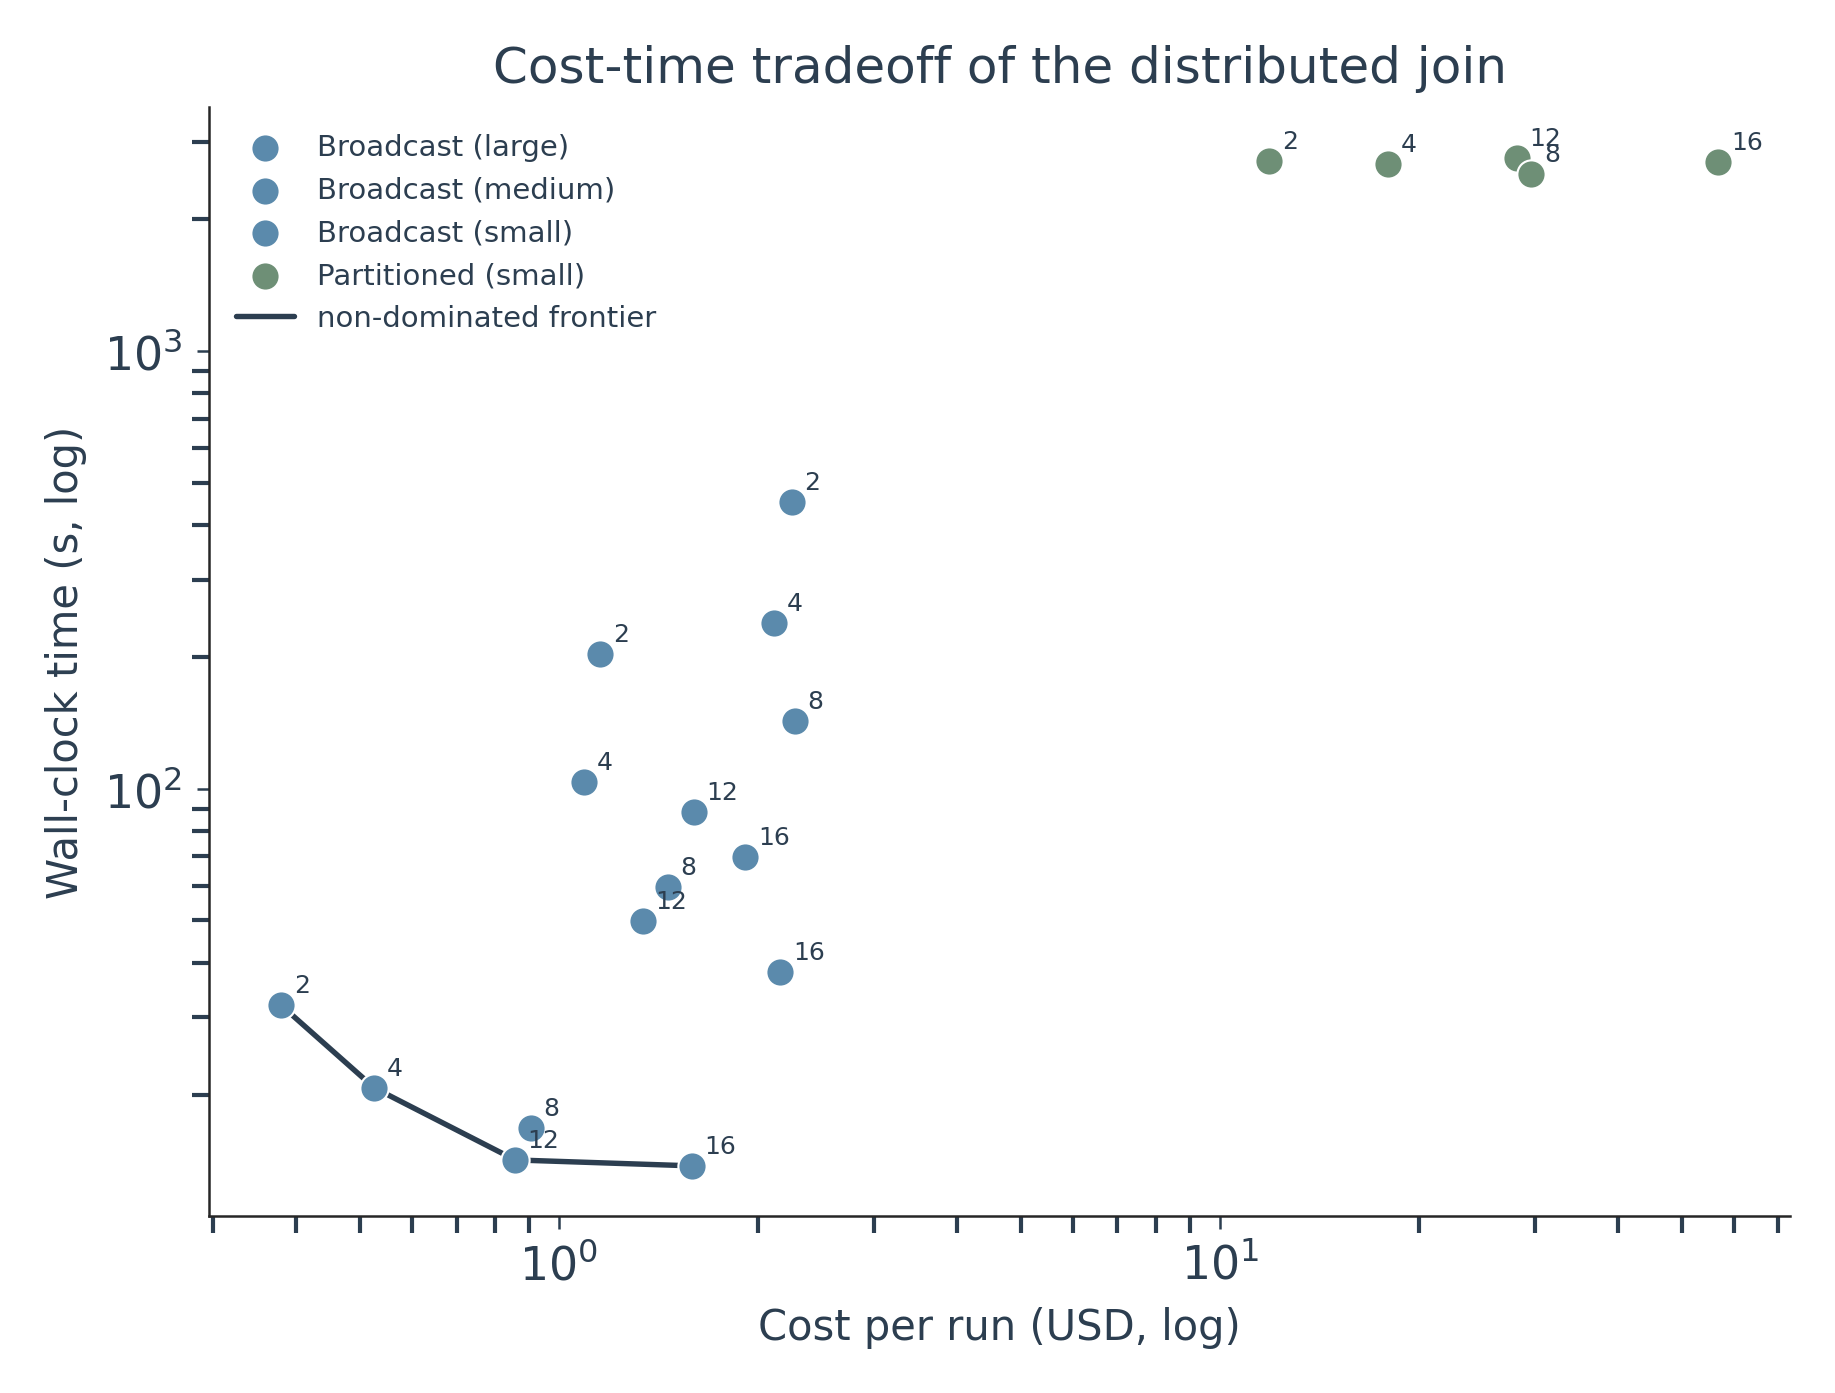
\includegraphics[width=0.75\textwidth]{Chapters/06-results/sub-chapters/figures/06-distributed-cost-time-pareto.png}
    \caption[Cost-time tradeoff of the distributed join]{Operational cost against
    wall-clock time for the distributed join, with one point per worker count and
    a separate series for each join strategy. The non-dominated points trace the
    cost-time Pareto frontier. Series colour encodes join strategy using the
    thesis palette.}
    \label{fig:distributed-cost-time-pareto}
\end{figure}

\begin{table}[H]
    \centering
    % WHAT IT SHOWS (supplementary): descriptive statistics of the distributed
    %   join per (configuration x size tier x worker count): achieved n, minimum
    %   estimator, CI half-width, dispersion, and the cost terms.
    % CAPTION MUST STATE: the columns and units; the estimator and CI method.
    % DATA: leave every data row commented out -- do NOT invent numbers.
    % NOTE: if the grid overflows one page, convert table -> longtable.
    \footnotesize
    \setlength{\tabcolsep}{6pt}
    \renewcommand{\arraystretch}{1.2}
    \begin{tabular}{@{}l l r r r r r@{}}
        \toprule
        \textbf{Tier} & \textbf{Strategy} & \textbf{Workers} & \textbf{Achieved $n$} & \textbf{Min.\ (\si{\second})} & \textbf{CI half-width} & \textbf{Cost (USD)} \\
        \midrule
        % TODO: one row per (tier x strategy x worker count). Example shape only,
        % no real numbers -- fill from run metadata:
        % Large & Broadcast   & 2  & <n> & <min> & <hw> & <cost> \\
        % Large & Partitioned & 16 & <n> & <min> & <hw> & <cost> \\
        % ...
        \bottomrule
    \end{tabular}
    \caption[Distributed join descriptive statistics]{Descriptive statistics of the
    distributed join for each size tier, join strategy, and worker count: the
    achieved iteration count, the minimum-estimator elapsed time, its bootstrap
    confidence-interval half-width, and the associated operational cost.}
    \label{tab:distributed-join-descriptive-statistics}
\end{table}
